\chapter{Implementation}\label{ch:implementation}
This chapter describes the implementation of \benchmark and the technologies used to realise the concepts introduced in Chapter \ref{ch:methodology}. While the methodology focused on the design decisions and theoretical foundation of the benchmark, this chapter examines how these ideas are put into practice in more detail. It explains the internal processing pipeline, how scenarios are constructed, how agent integration works, and how results are presented.



\section{Internal Processes}\label{sec:int-processes}
When running \benchmark, configurations in the form of YAML files are passed as input. These define the scenarios for evaluation, what agent to use (see more in Section \ref{sec:agent-integration}), which task to do and other settings. Listing \ref{lst:yaml-configs} shows a minimal working example for the configuration files. There, the IEEE 14-bus and 30-bus power grids are chosen, with the first and 100th profile indices for evaluation (see more on the Power Grids and Profiles in Section \ref{ssec:implementation-grid-profiles}). In the main configuration, the one on the right, a greedy agent is chosen that runs the tasks "Run" and "Evaluate" with four CPUs and with $N-1$ power flow calculation in the simulations. The greedy agent is configured with a reward function that minimises the maximum line loadings in $N-0$. The reward function is explained in more detail in Section \ref{sec:agent-integration} and the exact information on benchmark usage and what to set in the YAML files is shown in the documentation\footnote{\documentation} of the benchmark tool.

\begin{listing}[htp]
\centering
\footnotesize
\begin{minipage}{0.85\textwidth}
    \begin{minipage}[t]{0.32\textwidth}
    \begin{minted}{yaml}
- category: IEEE
  case: 14
  indexes:
    values: [0, 99]
- category: IEEE
  case: 30
  indexes:
    values: [0, 99]
    \end{minted}
    \end{minipage}
    \hspace{0.1\textwidth}
    \begin{minipage}[t]{0.47\textwidth}
    \begin{minted}{yaml}
name: "Greedy Agent"
agent_type: Greedy
scenario_files:
  - some/path/scenario.yaml
output_dir: some/path/output
task: ["Run", "Evaluate"]
n_cpu: 4
env_config:
  nminus1: True
  reward:
    max_line_loading_nminus0: 1.0
    \end{minted}
    \end{minipage}
\end{minipage}
\caption{Example YAML files for the benchmark settings: scenario (left) and main configuration (right)}
\label{lst:yaml-configs}
\end{listing}

Figure \ref{fig:bm-tasks} shows the processes inside \benchmark, which include the run and evaluation tasks that were previously discussed. Inside these configurations, the tasks that are set tell the benchmark tool what to do in the current run. Depending on these settings, either the main benchmark pipeline starts, or the results of already generated scores are presented (more on this in Section \ref{sec:result-format}). 

There are multiple processes that can be run inside the benchmark pipeline, each of which is run on all the chosen scenarios in the configuration. Before benchmarking starts, each scenario must be prepared. This is an important step for custom user agents, as training takes place here. This is discussed further in Section \ref{sec:agent-integration}. Once this step is complete, the agent runs through all scenarios separately. This is achieved using the PPTopoGym environment, which was presented in Section \ref{ssec:grid-ctrl-systems}. In this environment, the agent selects actions that are then executed, and the resulting state and reward are calculated using pandapower and a customisable reward function. If $N-1$ power flow calculation is set, like in Listing \ref{lst:yaml-configs}, then PPTopoGym performs these calculations using pandapower. The run either ends when the episode length is reached or when the power grid exceeds its limit and does not converge. Information about the run is always saved in the output folder, hence the user is able to skip this step, if they already have run data. This data is used for two final tasks. The evaluation task involves replaying the run data and gathering metrics to create the actual score. These metrics are then transformed into scores ranging from 0 to 100, which are then aggregated to produce a final score, as explained in Section \ref{ssec:score-calc}. Metrics for runtime per iteration, CPU usage and memory usage are measured during the run process. The evaluation data is then saved in JSON files, which document all the metrics and score pairs gathered for each scenario. These files are loaded by the result presenters shown in Section \ref{sec:result-format} to provide users with an overview of the benchmark output.

Another task that uses the run data is the replay task. In this task, the agent's actions are repeated in PPTopoGym, with plots and tables being created at each step of the episode. At the end of the task, these plots and tables are combined into an HTML file, which is then saved locally. This file provides a step-by-step visualisation of the actions chosen by the agent and their impact on the power grid in one run of a scenario. More about this output is discussed in Section \ref{ssec:replay-data}.

\begin{figure}[htp]
    \centering
    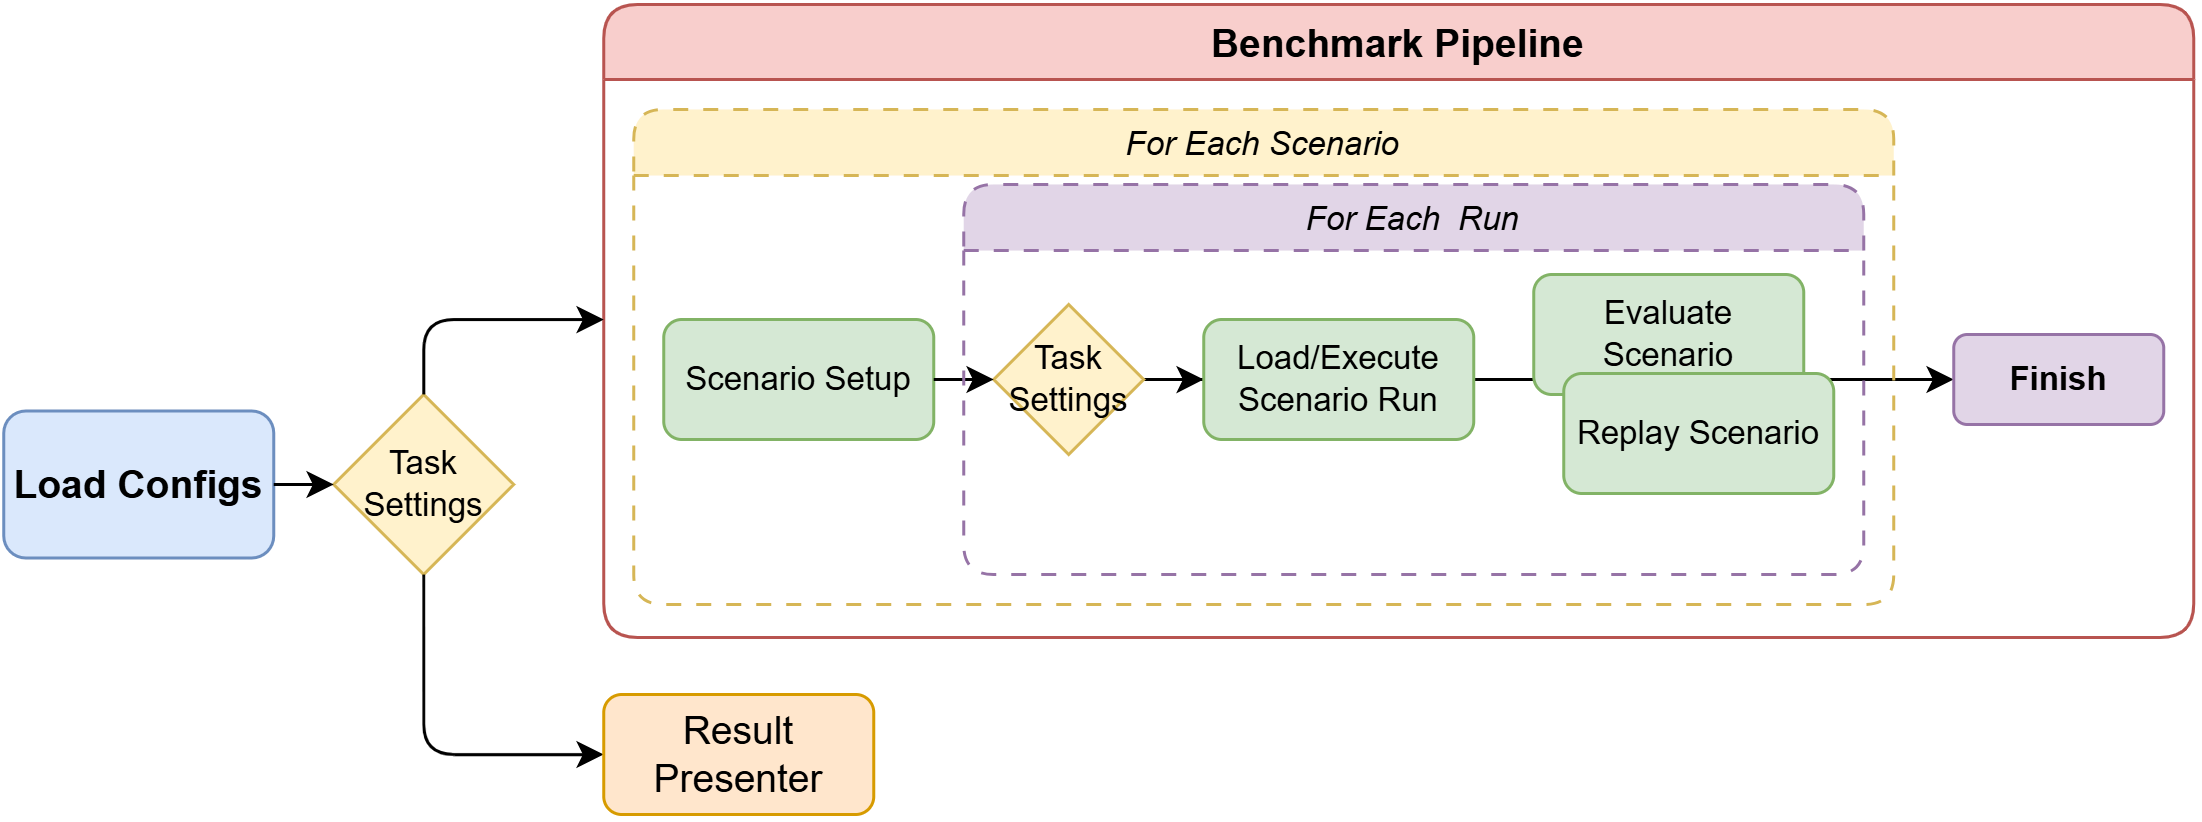
\includegraphics[width=0.95\textwidth]{images/implementation/benchmark_pipeline.png}
    \caption{Activity diagram showing all possible processes of \benchmark}
    \label{fig:bm-tasks} 
\end{figure}



\section{Scenario Implementation}\label{sec:implementation-scenarios}
This section describes how the scenarios introduced in Section \ref{sec:benchmark-structure} are implemented in \benchmark. It first presents the possible power grids and profiles that form the basis of a scenario. It then introduces the grid modifications that can be applied on top of these grids and profiles to increase scenario diversity and difficulty. Together, both define the building blocks to allow users to configure a wide range of scenarios.

\subsection{Grid and Profiles}\label{ssec:implementation-grid-profiles}
As discussed in Section \ref{sec:benchmark-structure}, each scenario consists of a power grid, a profile, and network modifications. Currently, the power grid benchmark supports IEEE test cases and data from SimBench. 

The IEEE test cases are introduced in Section \ref{ssec:power-benchmark}, as standardised and realistic power grid models. Figure \ref{fig:exp-grids} shows the 14-bus and 30-bus grids from the IEEE test cases, which are used in the experiments in Chapter \ref{ch:experiments}. They contain buses (shown as the circles), loads and generators (depicted as green and red triangles), transmission lines and transformers (represented as lines, with transformers drawn thicker), and the external grid (illustrated as the yellow rectangle). While pandapower does not have any substation modelling, PPTopoGym supports it by adding substation information to a pandapower grid \cite{pptopogym}. External grids in pandapower are modelled as voltage sources with a defined voltage magnitude and angle, which are represented as slack nodes in the power flow calculation and thus balance the power in the grid \cite{pandapower}.

SimBench is a benchmark dataset of German power grids, which provides realistic grids and profiles with 15-minute resolution over the course of a full year. It offers thirteen different power grids, each with three variants, as well as a variety of profiles (e.g. for photovoltaic or wind generation) \cite{simbench}. Additionally, SimBench data supports the format used in pandapower \cite{simbench}, making it a fit usage in PPTopoGym. 

The IEEE test cases have been selected because they have been used in many previous studies for benchmarking power grids, and because they are realistic. The SimBench dataset has been selected to complement the limited number of IEEE test cases and to provide more variety and benchmark coverage. Both datasets model realistic grid topologies ranging from small to large power grids, with profiles always loaded from the SimBench dataset.

\subsection{Grid Modification}\label{ssec:implementation-grid-mod}
To create a broader variety of scenarios for testing the agents, \benchmark offers a few network modifications that users can configure. These modifications make scenarios more or less complex in terms of grid stability, depending on the scaling. This allows the agent to be pushed to its limits more effectively, enabling a deeper assessment of its strengths and weaknesses and creating edge cases for evaluation. The modifications include load and generator scaling, maintenance events, and line and transformer capacity scaling.

\paragraph{Load and Generator Scaling.} Load and generator scaling redistributes the consumption or generation of electricity. This allows scenarios to be created where most of the electricity comes from a few generators or where a couple of loads require much more electricity than the rest. This maintains the total amount of electricity generated and consumed from the original data, but shifts the distribution to be more or less extreme.

\paragraph{Maintenance Events} Another modification is the introduction of maintenance events, which simulate real-world situations in which grid components are turned off due to maintenance or outages caused by long-term usage. These components include lines, switches, transformers and generators. This feature is similar to the maintenance in the \ac{l2rpn} benchmark explained in Section \ref{sssec:l2rpn}. Scenarios involving maintenance are more challenging as electricity must flow through longer paths or generation relies on fewer generators. Furthermore, to make the simulation more realistic, transmission lines or transformers, that reached a loading of 150\% of their physical limit, get set into maintenance. This simulates edges of the grid that were pushed over the limit and were destroyed in the process. When that happens, they need to be fixed, hence the maintenance event. They will not be usable for the rest of the episode. 

\paragraph{Line and Transformer Capacity Scaling} The capacity of lines and transformers is scalable, to configure the maximum allowed current of lines and transformers. This adjusts how fast the physical limit of the grid edges is reached. This is done by scaling the \textit{max\_i\_ka} value, which is the maximum allowed current in kiloamperes \cite{pandapower_docs}. If the value is reduced, the lines and transformers reach their thermal limits faster. This is relevant in grids where a specific line or transformer is particularly important. When the capacity of this component is reduced, the agent must distribute the electricity to other components. Otherwise the downscaled component may fail due to exceeding its limit for too long.



\section{Agent Integration}\label{sec:agent-integration}
\benchmark offers two baseline agents and allows users to implement their own. The first baseline is a \textbf{do-nothing agent}, which never applies any action to the power grid. The second is an exploitative \textbf{greedy agent}, which evaluates the available actions in the current state and selects the one yielding the highest reward.

The reward signal is provided by the underlying PPTopoGym environment from the work of \citet{pptopogym} and is therefore not part of the benchmark contribution of this thesis. However, the function was extended into a configurable, metric-based form used for the experiments shown in Chapter \ref{ch:experiments}. Equation \ref{eq:reward_func} defines this reward. If the power flow does not converge in the current step, the reward is the constant penalty $r_{\mathrm{fail}}$. Otherwise, it is computed as a weighted sum of metric scores. Each metric $m \in \mathcal{M}$, with $\mathcal{M}$ being the set of reward metrics in use, corresponds to a value measured from a grid feature and is weighted by $w_m$. The scoring function $s_m$ maps the measured value to $[0,1]$ using a worst-case and a best-case reference value, clipping results that fall outside this interval. Normalising by the sum of the absolute weights yields a reward in $[0,1]$. The available metrics and reference values partly coincide with the benchmark metrics of Section \ref{sec:metrics-eval}. In the benchmark configuration, the user sets which reward metrics to use and how much weight they have. Section \ref{ssec:reward-metrics-description} lists the configurable options for the reward and what their worst-case and best-case reference value, for the score mapping, are set to.

\begin{equation}
\text{reward} =
\begin{cases}
r_{\mathrm{fail}}, & \text{if the power flow does not converge},\\[2.2ex]
\displaystyle \frac{\sum_{m \in \mathcal{M}} w_m \, s_m}{\sum_{m \in \mathcal{M}} \lvert w_m \rvert}, & \text{otherwise}.
\end{cases}
\label{eq:reward_func}
\end{equation}

Another type of agent is custom agents brought by the user. These, just like the greedy agent, use the customisable reward function from Equation \ref{eq:reward_func}. In order to create such a custom agent, a couple of inputs and outputs need to be implemented. The \texttt{BenchAgent} class within the project defines this structure. Custom agents must be a subclass of the \texttt{BenchAgent} class. The necessary functionalities are shown in Figure \ref{fig:agent-pipeline}. The custom agent is embedded in the benchmark pipeline discussed in Section \ref{sec:int-processes}, where it is connected to the benchmark setup and scenario execution. For the setup, a \ac{rl} agent needs to be initialised and then trained for each scenario. During training, the agent produces checkpoints which save the trained state after multiple iterations. It is possible to use these to either skip the training process and load an existing checkpoint, or ensure reproducibility with the same state as a trained agent. Once the agent has been set up for one scenario, it is used to decide on actions during evaluation runs. After these runs have been saved, the agent can be evaluated, or the actions can be replayed. Additionally, \benchmark offers a \texttt{RayAgent}, a child class of \texttt{BenchAgent} that provides multiple RLlib-implemented functionalities. RLlib is a \ac{rl} library built on top of the Ray framework. It offers a unified interface and implementation of \ac{rl} algorithms, such as \ac{ppo} \cite{rllib}. The \texttt{RayAgent} class simplifies the process of creating a new agent, as only agent initialisation needs to be implemented. 

\begin{figure}[htp]
    \centering
    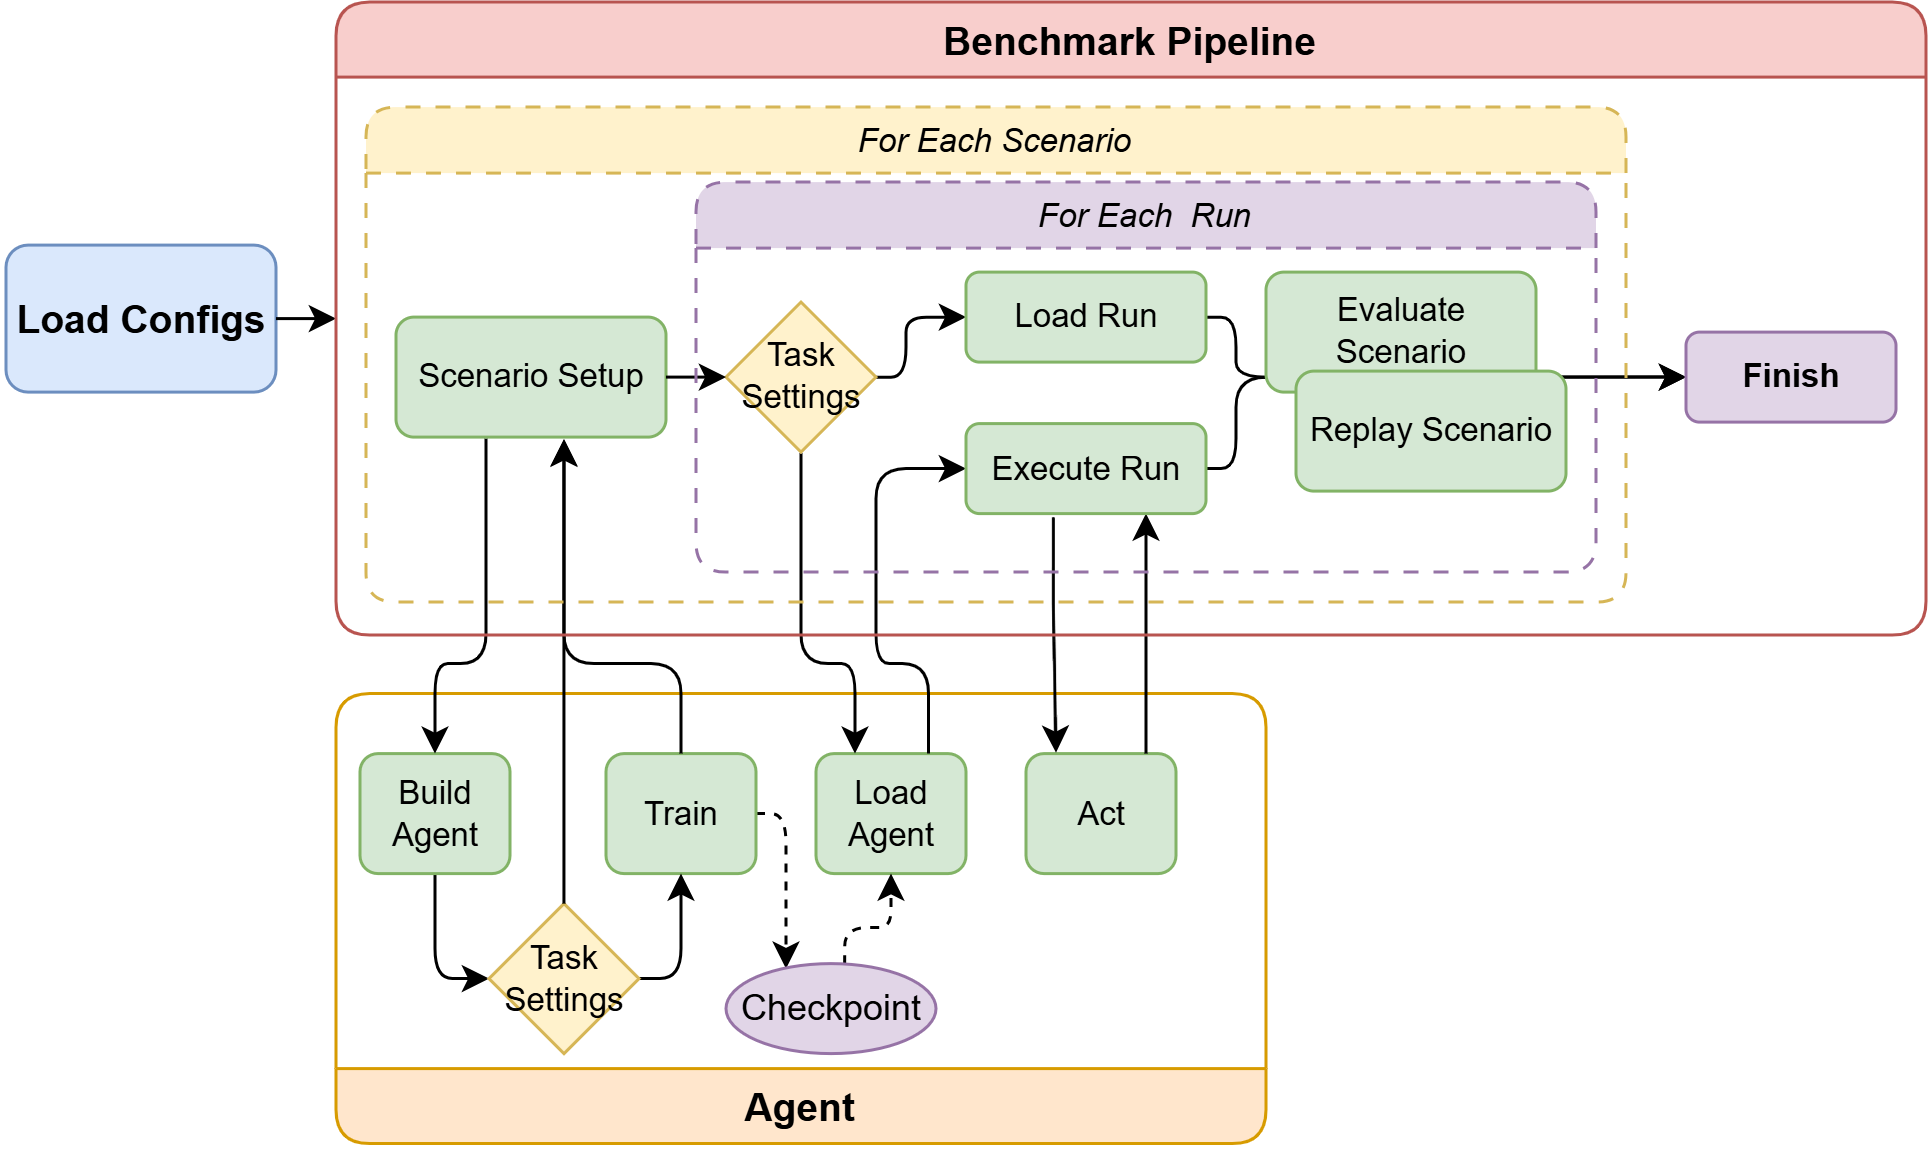
\includegraphics[width=0.95\textwidth]{images/implementation/pipeline_agent.png}
    \caption{Interaction between the benchmark pipeline and the agent}
    \label{fig:agent-pipeline} 
\end{figure}

\ac{rl} agents do not optimise every parameter during training. Hyperparameters, such as the learning rate, layers in a neural network, or the batch size, are set during initialisation and never changed. To find the perfect settings for these, \benchmark offers the \texttt{BaseTuner} class. This class provides an interface for custom tuning classes that optimise the hyperparameters of custom agents. A child class of \texttt{BaseTuner} is \texttt{OptunaTuner}, which simplifies the implementation of custom Optuna tuning for the user's agent. Optuna is a hyperparameter optimisation framework \cite{optuna}. The user defines the value ranges for each hyperparameter in the custom child class of the \texttt{OptunaTuner}. Optuna then creates the search space, carries out the experiments, and returns the optimal hyperparameters efficiently and reproducibly \cite{optuna}.



\section{Result Format}\label{sec:result-format}
This section demonstrates how the evaluation output is visualised and which tools are offered to do so. The format of the results and the information shown affect the quality and focus of the feedback provided to the user. Some important information is not immediately apparent and requires the correct visualisation to be seen. Furthermore, the benchmark gathers a lot of information, which would be time-consuming to read and analyse. The following paragraphs will present how the raw output, which contains a lot of information, is summarised and visualised to provide an in-depth overview of the agent's performance using textual or visual feedback.

\subsection{Raw Output}\label{ssec:raw-output}
Once an agent has been evaluated, the resulting metrics and scores are saved in a JSON output. The output for each scenario looks like the example in Listing \ref{lst:result-json}. Each run of the scenario is saved in the \texttt{results} array. All the metrics for each of these runs are saved as value-score pairs. For example, for the metric \texttt{timesteps\_without\_overload} of the first result in the example, there were zero timesteps with any overloads over the full episode with 96 timesteps, giving the best score of 100. Some metrics have multiple values, such as the total number of lines overloaded per timestep in $N-0$ power flow (shown here as \texttt{\seqsplit{total\_lines\_overloaded\_timestep\_nminus0}}), for which the value-score pairs for each iteration are saved. For these metrics, the mean and worst scores are used to aggregate the scores into a single score. This is saved in \texttt{resulting\_scores}, and the measured values for these scores are in \texttt{resulting\_values}. When only one value is measured for a metric, such as timesteps without overload, there is only one resulting score and value. To understand the scoring from 0 to 100, the worst and best possible values are stored in \texttt{scoring\_range}.
Once all the metrics have been listed inside a category, the category score is saved. This is done for each category in the same way, unless a category has a weight of zero. In that case, as can be seen in the computational performance category of the example, no metrics are measured or saved, and only a category score of zero is written. Finally, the index, episode length and the aggregated score are saved for each run.

\begin{listing}[htp]
\begin{minted}[fontsize=\scriptsize, breaklines, baselinestretch=0.6]{json}
{
    "name": "IEEE14_original",
    "network_category": "IEEE",
    "scenario_config": ".../ieee14.yaml",
    "results": [
        {
            "overload_mitigation": {
                "timesteps_without_overload": {
                    "values": [[96.0, 100.0]],
                    "resulting_scores": 100.0,
                    "resulting_values": 96.0,
                    "scoring_range": {"wp_val": 96.0, "bp_val": 0.0}
                },
                ...
                "total_lines_overloaded_timestep_nminus0": {
                    "values": [[0.0, 100.0], [0.0, 100.0], ...],
                    "resulting_scores": {"mean": 100.0, "worst": 100.0},
                    "resulting_values": {"mean": 0.0, "worst": 0.0},
                    "scoring_range": {"wp_val": 15.0, "bp_val": 0.0}
                },
                ...
                "category_score": 89.64805329153604
            },
            "voltage_violation_mitigation": { ... },
            "survival": {
                "survived_iterations": {
                    "values": [96.0, 100.0],
                    "resulting_scores": 100.0,
                    "resulting_values": 96.0,
                    "scoring_range": {"wp_val": 0.0, "bp_val": 96.0}
                },
                "category_score": 100.0
            },
            "costs": { ... },
            "computational_performance": {"category_score": 0.0},
            "index": 1920,
            "episode_length": 96,
            "total_score": 83.70538341352134
        },
        ...
    ]
}
\end{minted}
\caption{Exemplary output for the do-nothing baseline agent.}
\label{lst:result-json}
\end{listing}

After gathering the data for each scenario result, \benchmark creates a \textit{statistics.json} file, which summarises the total and scenario results. Listing \ref{lst:statistics-json} illustrates an example of what this might look like. It presents information about the final aggregated score, the average category score, and the number of metrics gathered across all scenarios. In this case, there were 15 scenarios, each measuring 27 different metrics, for a total of 810 metrics measured across all 30 runs. Additionally, the same information is shown for each scenario. 

\begin{listing}[htp]
\begin{minted}[fontsize=\scriptsize, breaklines, baselinestretch=0.6]{json}
{
  "total_score": 64.8135,
  "category_scores": {
    "overload_mitigation": 69.1923,
    ...
  },
  "metrics_average": {
    "timesteps_without_overload": {"score": 20.6598, "value": 19.8333},
    "total_lines_overloaded":     {"score": 99.1886, "value": 32.0},
    ...
  },
  "metrics_gathered": {
    "amount_of_metrics": 27,
    "amount_of_scenarios": 15,
    "total_amount_metric_gathered": 810
  },
  "scenarios": {
    "IEEE14_original": {
      "scenario_score": 52.7911,
      "category_scores": {
        "overload_mitigation": 89.7843,
        ...
      },
      "metrics_average": {
        "timesteps_without_overload": {"score": 0.0,    "value": 0.0},
        "total_lines_overloaded":     {"score": 100.0,  "value": 0.0},
        ...
      },
      "metrics_gathered": {"amount_of_metrics": 27, "total_amount_metric_gathered": 81}
    },
    "IEEE14_upscale_gen0_downscale_rest": {
      "scenario_score": 40.4203,
      ...
    },
    ...
  }
}
\end{minted}
\caption{Exemplary \textit{statistics.json} output for the do-nothing baseline agent.}
\label{lst:statistics-json}
\end{listing}

JSON is a human-readable output format, but it quickly becomes overloaded with text and information when dealing with large amounts of data. Moreover, to make the data more compact, not all the data is labelled or explained. For example, the saved values are value-score pairs, which are not explained anywhere. The main purpose of this output format is to save the evaluation on the machine for later analysis.

\subsection{Textual Feedback}\label{ssec:textual-feedback} 
\benchmark offers two forms of textual feedback, which share the same information. One creates a report that is printed in the console and saved in Markdown format. An example of the console printing is demonstrated in Listing \ref{lst:textual-report}. This shows the results for a do-nothing agent that went through 15 different scenarios and a total of 30 runs across all scenarios. 
Initially, this information is presented, including the average general score and average category scores. Then more specific information is displayed, such as average scores and measured values for specific metrics, and how often these were gathered throughout the experiment. Additionally, the average scenario scores and the number of runs are shown. Finally, the report goes through each scenario, providing average scores for the categories and metrics. Alternatively, there is an interactive reporter where the user selects which of this information should be printed in the console using console inputs. The textual feedback form is useful for quickly obtaining a thorough overview of the average values and scores across multiple levels within the benchmark. It produces output similar to JSON files, but in a more readable and compact format. 

\begin{listing}[htp]
\begin{minted}[fontsize=\scriptsize, breaklines, baselinestretch=0.6]{text}
============================================================
BENCHMARK REPORT: DN
============================================================
Agent:               DoNothing

OVERVIEW
----------------------------------------
Average Score:       64.8135
Total Scenarios:     15
Total Results:       30
Category · overload_mitigation:          69.1923
...

METRICS OVERVIEW
----------------------------------------
Metric                                    Avg Score  Avg Value  # Gathered
timesteps_without_overload                  20.6598    19.8333          30
total_lines_overloaded                      99.1886    32.0000          30
...

SCENARIO OVERVIEW
----------------------------------------
Scenario                                Avg Score  # Gathered
IEEE14_original                           42.7911           3
IEEE14_upscale_gen0_downscale_rest        40.4203           2
...

------------------------------------------------------------
Scenario: IEEE - IEEE14_original
------------------------------
Configuration:  .../ieee14.yaml
Network Category:    IEEE
Average Score:       42.7911
Category · overload_mitigation:          89.7843
...

Metric Overview
------------------------------
Metric                                    Avg Score  Avg Value  # Gathered
timesteps_without_overload                 100.0000     0.0000           3
total_lines_overloaded                     100.0000     0.0000           3
...
\end{minted}
\caption{Exemplary benchmark report for the do-nothing baseline agent.}
\label{lst:textual-report}
\end{listing}

\subsection{Visual Feedback}\label{ssec:visual-feedback}
Another type of result is graphs and plots. These enable users to instantly identify trends, distributions and comparisons. This makes them especially valuable for determining which scenarios or categories an agent is struggling with and for comparing multiple agents against each other.

\subsubsection{Result Plots}
The output of the plotting tool is created using Matplotlib, a Python library for creating publication-quality static plots and graphs \cite{matplotlib}. Additionally, as an alternative to Matplotlib, the plotting tool offers Plotly, which is another Python library for creating interactive plots and graphs \cite{plotly}. The same plots are created for both Matplotlib and Plotly. These include five overview plots containing all scenarios, and three plots showing how the agent performed in each scenario.

Figure \ref{fig:eval-plots} illustrates an example of all the overview plots. It contains a heatmap presenting the score for each category in each scenario, the distribution of scores across all runs in each scenario, the distribution of category scores, and a comparison of scores across scenarios and their individual runs. These plots help to visualise the strengths and weaknesses of the agent in each category or scenario. In the presented example, it can be seen that the agent performs very well in terms of overload mitigation, but struggles with voltage violations. Furthermore, the agent performs much better in the \texttt{IEEE14\_upscale\_load0\_downscale\_rest} scenario, in which the 14-bus power grid from the IEEE test cases is used and modified so that load 0 has an increased power demand.

Figure \ref{fig:eval-scenario-plots} demonstrates an example of the individual scenario plots. These plots include a radar chart of the category scores, the category scores themselves, and the total score for each run. The plots again show, that voltage violation was the agent's weakness and overload mitigation its strength for this scenario. Additionally, they demonstrate that the category scores and the average score in the first and third runs, as shown in Figures \ref{fig:eval-category-bar} and \ref{fig:eval-score-index}, are higher than in the second scenario run.

\subsubsection{Webapp}
Another supported visualisation is an interactive web app with Streamlit. Streamlit is a Python framework for building lightweight web applications that focus on data presentation \cite{streamlit}. Figure \ref{fig:webapp-screenshots} depicts screenshots of an example result from a web app created for an experiment involving a do-nothing agent. The web app combines textual and visual reports similar to those demonstrated previously. It begins with an overview, shown in Figure \ref{fig:webapp-overview}, where the user sees a summary of how well the agent performed overall. This includes information about the average score, the number of scenarios and the total number of runs, as well as the average scores for each category. The scenario overview and scenario details then provide information about each scenario, including the average score, the number of runs, and the average category scores. This allows for individual scenario analysis to identify which ones were more difficult to solve. 
Finally, the section on individual results goes over each run of the currently selected scenario in the section on scenario details, presenting the average score and the score over categories and metrics. These metrics and scores provide the lowest level of detail and are used to analyse specific runs in greater depth. The web app shows the same plots for each scenario as in Figures \ref{fig:eval-scenario-plots} and \ref{fig:eval-plots}, using either Plotly or Matplotlib. In this way, the web app provides in-depth analysis of specific scores or runs and visual representations using plots from the plotting tool. This makes it easier to analyse strengths and weaknesses, as well as provide an overview of the agent. Users are able to perform both superficial and general performance analyses, as well as conduct more in-depth analysis to identify the root causes of problems. 

So far, the result format has focused on feedback for single-agent experiments, but the web app additionally has an option to start a comparison between two agents. This is built similarly to the standard web app, but it displays the results side by side, as depicted in the example in Figure \ref{fig:comparison-webapp-screenshots}. Additional features include demonstrating differences in scores and plotting category scores next to each other for direct comparison of the two results. This form of feedback is useful for comparing two agents. It provides a general comparison using the aggregated scores and a specific comparison for individual runs or scenarios using generated plots displayed side by side. This makes it easy to see which agent has stronger or weaker features, making the decision between the two agents easier.

\subsection{Replay Data}\label{ssec:replay-data}
One form of feedback that does not use evaluation data to generate its output is data from the replay task. As explained in Section \ref{sec:int-processes}, this data is created by replaying the run data and constructing plots of the state of the power grid at each timestep. The plots are created using Plotly, and the output is an HTML page containing all the information in one page. The page contains two graphs at the beginning, both of which illustrate the power grid from different perspectives. Below these, there is a section demonstrating all the tables from the pandapower network (lines, buses, generation, etc.). Figure \ref{fig:replay-graphs} shows how the two graphs make up this page.

Figure \ref{fig:network-graph} shows a network graph that visualises the grid's topology and indicates how close each component is to its operational limit. For example, the colours green to red to black on the transmission lines illustrate how much they are overloaded. Red or black indicates that the line is overloaded by more than 100\%. The same is done for transformers, if any exist. For the buses, the normalised bus voltage is presented to indicate how much it deviates from the operational safe range. Green indicates normal voltages, while shades of blue or red demonstrate that the voltages deviate too far below or above the nominal values. The darker the colour shades, the worse the voltage violations. Additionally, this graph shows which generator produces the most power and which load consumes the most, highlighting them in a darker shade of their respective colour.

The action graph, as shown in Figure \ref{fig:action-graph}, focuses more on the actions taken by the agent. It demonstrates which bus was affected by the agent's action, such as the topology changes that were made. An example of this is demonstrated in Figure \ref{fig:action-graph-zoomed}, which is the same grid as in Figure \ref{fig:action-graph}, just zoomed in. This figure shows how one bus was split and which lines were connected to which of the new buses. Moreover, it illustrates how the load, labelled \textit{L2} in this plot, was connected to the substation on the right-hand side of the figure. As the plots are created using Plotly, it is easy to zoom in and analyse the new grid connections made after an agent's action.

This output is an analysis tool that helps users to understand the actions of agents and their impact. If a user, for example, is unsure why the agent received a low score in a specific category, the option to use the replay data exists. This helps identify the behaviour or actions that caused the agent to perform poorly in that category. Furthermore, this output is useful for identifying challenging scenarios to use for benchmarking. It provides a visual analysis, demonstrating for each step of an episode which lines are the bottlenecks, which generators produce more, and which loads require more power. Unlike the others, this output uses different data and has a different goal. It analyses past runs to provide insight into the grid and the agent by showing actions, bus splits and how the grid reacts to new states.